\chapter{Bidirectional Encoder Representations from Transformers}
\label{sec:bert}

Bidirectional Encoder Representations from Transformer~(BERT) is a language model that has produced state-of-the-art results for several natural language processing tasks~\cite{devlin2018bert}. Previous recurrent models such as Long Short-Term Memory~(LSTM) compute hidden states of an input sequence sequentially, whereby each hidden state depends on the state of the previous hidden state. Consequently, this mechanism prevents the parallelization of training long input sequences~\cite{vaswani2017attention}. In contrast, BERT can learn the context of input sequences more efficiently, as it can process every item in the sequence in parallel in all layers. BERT is therefore aware of both the left and the right context of a sequence at all times, by using a novel deep bidirectional transformer architecture. In this chapter, we are going to explain the mechanics of BERT. The embedding and representation of input sequences, the self-attention, and multi-attention mechanism for understanding the context of a sequence, as well as the pre-training tasks to train the model. As we will explain in Section~\ref{sec:bert_recommendations}, we can exploit BERTs capabilities to learn about the context of sequences to make recommendations.


\section{Input Embeddings}
\label{sec:embeddings}
The first component of the BERT architecture is the embedding of input sequences. Arbitrary objects need to be turned into a common representation that the model can understand. For simplification, we will present the embedding of words and sentences, as this is the most common use case for BERT, but we can feed arbitrary sequences of objects to BERT as we will demonstrate in the section~\ref{sec:bert_recommendations}

\paragraph{Tokenizer}
Every BERT model needs to have a unique tokenizer, that accepts sequences such as text sentences and turns them into tokens that serve as the input to the model. The tokenizer consists of a fixed-sized unique vocabulary where each token corresponds to an embedding vector with a fixed size.  

The original BERT model trained by Google contains roughly 30000 words and subwords chosen based on frequency from Wikipedia and a large corpus of books. In case a word is not in the vocabulary, the tokenizer breaks it down into subwords. Since the vocabulary contains subwords for every character in the alphabet, we can tokenize words, that are not in the vocabulary. By using more subwords and fewer whole words, the vocabulary becomes smaller, and training efficiency increases. Figure~\ref{fig:bert_tokenizer} shows the example code of the tokenizer for the original BERT base model trained by Google. The Tokenizer breaks down the words that are not in the vocabulary into subwords. All subwords are prefixed with two pound signs.

\begin{figure}[htbp]
\centering
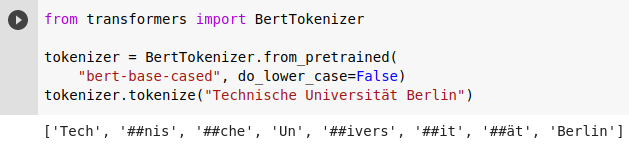
\includegraphics[width=0.9\textwidth]{images/illustrations/bert_tokenizer.png}
\caption{An example showing the BERT Tokenizer for the original BERT base model trained by Google. The Tokenizer breaks down the words that are not in the vocabulary into subwords. Every subword is prefixed with two pound signs.}
\label{fig:bert_tokenizer}
\end{figure}

\paragraph{Reserved Tokens}
The BERT neural network architecture requires fixed-length inputs. Since sequences are of arbitrary length, the BERT tokenizer adds [PAD] tokens to the end of the sentence to pad it to the fixed-length required by the model. A limitation of the model is a maximum sequence length of 512 items. There are three more reserved tokens. The [SEP] token separates a sentence into two parts. This token is necessary for the "next sentence prediction" task. The [MASK] token is used for the "masked language model" task. We will describe both tasks in section~\ref{sec:transformer}.
Another reserved token is the [CLS] token. By default, the [CLS] token is added at the first position of every sequence. It is a classifier token that produces a binary output at the last layer of the model and is essential for the "next sentence prediction task".

\paragraph{Positional Embeddings}
Unlike recurrent neural network models, that process one word at a time, BERT processes all words in parallel, thus requiring a notion of word order. To achieve this, BERT adds a positional encoding vector to each item of the sequence, at layer one.


\section{The Transformer and Multi-Head Attention}
\label{sec:transformer}

\begin{figure}[htbp]
\centering
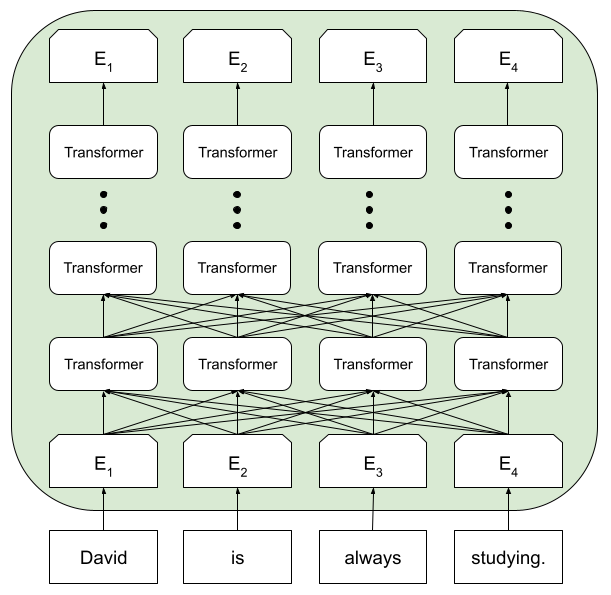
\includegraphics[width=0.85\textwidth]{images/diagrams/bert_layers.png}
\caption{The BERT model. After the words are tokenized, the first transformer layer takes the word embeddings, processes them in parallel and amplifies them. This process is repeated 12 times. The input and output dimensions are the same.}
\label{fig:bert_layers}
\end{figure}

\paragraph{BERT Layers}
At first, the tokenizer splits a sequence and turns it into word embeddings. Then the word embeddings get passed through 12 layers.
Each layer contains a Transformer that learns about the relationship and context of items in the sequences and outputs augmented word embedding to the next layer. We will explain the Tasks to train the model in section~\ref{sec:bert_tasks}. Figure~\ref{fig:bert_layers} shows the basic structure of the BERT model, including the 12 Transformer layers. The fully connected lines between the different layers indicate that BERT processes the embeddings in parallel and therefore in a fully context-aware manner.

\paragraph{The Transformer}
To understand how BERT can learn about the context and relationship of items or words in a sequence, we need to look at the Transformer model. The Transformer is a model developed and presented by Google in a paper called "Attention is all you need"~\cite{vaswani2017attention}. Unlike previous models, it does not use any convolution or recurrence in its architecture. Instead, it proposes a novel attention-based architecture. The Transformer is a powerful model for machine translation, mainly due to its capability to parallelize the computation. It outperforms previous models for machine translation and is currently the key technology behind Google Translate~\cite{googleaiblog}. The Transformer consists of two components: an encoder and a decoder. BERT only uses the encoder component. By utilizing 12 layers of stacked encoders, BERT can learn about the context and relationship between the different item embeddings in a sequence. The encoder uses a novel attention mechanism to learn about the embedded items or words.  

\begin{figure}[htbp]
\centering
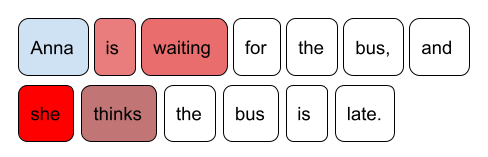
\includegraphics[width=0.9\textwidth]{images/illustrations/bert_self_attention_sentence.png}
\caption{An imaginary example sentence. The self-attention mechanism looks at a particular word, in this case, the word "Anna" and tries to find words that are associated, like the word "she" or "thinks"}
\label{fig:bert_self_attention_sentence}
\end{figure}

\begin{figure}[htbp]
\centering
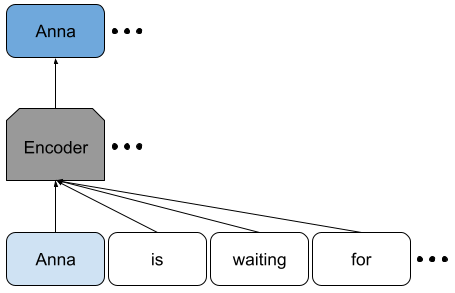
\includegraphics[width=0.7\textwidth]{images/illustrations/bert_self_attention_one_word.png}
\caption{An example encoder for the word "Anna". It looks at all the other word embedding and tries to encode the association into an amplified word embedding of "Anna" that gets passed on to the next layer.}
\label{fig:bert_self_attention_one_word}
\end{figure}

\paragraph{Self-Attention}
The Transformer and the Encoder component specifically use a novel self-attention mechanism to encode item embeddings. BERT consists of 12 layers of stacked encoders. We will describe the self-attention mechanism to see how BERT can learn details about items in a sequence. For simplicity, we will look at the mechanism, one word at a time, before we elaborate on how the process works in parallel using multi-headed attention. Depicted in Figure~\ref{fig:bert_self_attention_sentence} is an imaginary example sentence. In the example, we omit the tokenization into subwords. The self-attention mechanism looks at particular word embeddings. Suppose the encoder looks at the word "Anna", highlighted in blue. Sentence structures can contain parts such as adjectives, verbs, nouns, or adverbs. To learn more about the meaning of a sentence, we need to understand how words are associated to each other. For a human reader, it is easy to see that the pronoun "she" is relating to "Anna", and that "Anna" is "waiting" and "thinks". The words connected to the word "Anna" are highlighted in different shades of red. The task of the encoder is to encode into a specific word embedding the association to all other words in the sentence. An example in Figure~\ref{fig:bert_self_attention_one_word} shows the architecture of one single encoder. Every word has its own encoder. In this case, the encoder for the word embedding "Anna" looks at all the other word embedding and tries to encode the association into an amplified word embedding of "Anna" that gets passed on to the next layer. Self-attention stands for the degree of attention or focus to put on specific words during the encoding process.

\paragraph{Vector Calculation of Self-Attention}
We will now explain the mathematics behind the self-attention mechanism~\cite{vaswani2017attention,theillustratedtransformer}. Initially, the tokenizer splits the input sentence into subwords which are part of the vocabulary, and turns them into embedding vectors of size 768 as described in the section~\ref{sec:embeddings}. Next, the mechanism creates a query, a key, and a value vector for each word embedding. These vectors are just another representation, calculated by projecting the input embedding vectors to a different subspace. A value vector represents the content of an embedding. The query vector is used as an input query to calculate self-attention. We calculate query vectors against the key vectors. To obtain these vectors, we multiply each input embedding against projection matrices: A query, a key, and a value matrix all of size 768x768. Each of these matrices is formed and fine-tuned during the training process.

\begin{figure}[htbp]
\centering
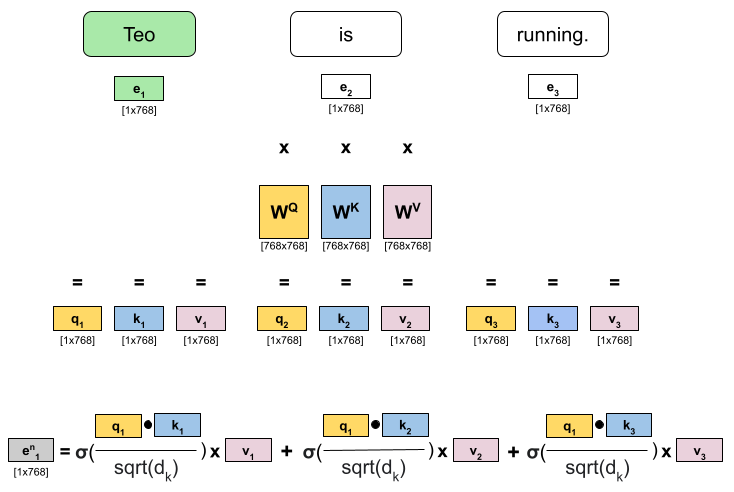
\includegraphics[width=1\textwidth]{images/illustrations/bert_self_attention_calculation.png}
\caption{Depicted in the drawing is the self-attention computation for the word "Teo". For every word embedding, we build a query, key, and value vector. Next, we compute the dot product between the query vector of "Teo" and all key vectors. We scale the resulting scores and apply the softmax function to every score. The final step is to multiply every score with the corresponding value vector and sum up the vectors. The result is the new embedding vector $e^n_1$ for the word Teo, which gets passed on to the next layer.}
\label{fig:bert_self_attention_calc}
\end{figure}

Before we demonstrate the calculation of self-attention in matrix form, which represents the actual implementation, we will describe it in vector form. Depicted in Figure~\ref{fig:bert_self_attention_calc} is another imaginary example sentence, again omitting the tokenization into subwords. The figure shows the self-attention calculation that the encoder does for the word "Teo". At first, the words in the sentence are tokenized into the embedding vectors $e_i$ and then transformed into the representing query, key, and value vectors: $q_i$, $k_i$, and $v_i$ by multiplying the embeddings with the query, key, and value projection matrices: $W^Q$, $W^K$, and $W^V$. 

Since we compute the self-attention for the word "Teo", we need to calculate its dot product between the query vector of "Teo" and every key vector from the other words in the sentence. This calculation gives us a score for every word in the sentence. The score tells us to what degree the word "Teo" is in association with the other words in the sentence. Hence it is a score of how much attention the encoder should give to each word that produces the new amplified encoding for the next layer.

Next, we divide each score by the square root of $d_k$, whereby $d_k$ is the dimension that the query, key, and value vectors have. This scaling of the scores leads to more stable gradients during training~\cite{vaswani2017attention}.

Now, the softmax function gets applied to all the scores. The softmax function $\sigma$ normalizes the scores so that the sum of all the scores adds up to 1. For $K$ many scores it is defined as follows~\cite{softmax}:

\begin{equation}
\setlength{\jot}{25pt}
    \begin{aligned}
    \sigma : \mathbb{R^K} \rightarrow [0,1]^K  \quad\quad
      \sigma(x)_i=\frac{e^{x_i}}
      {\sum\limits_{j=1}^K e^{x_j}}
    \end{aligned}
    \label{equation:softmax}
\end{equation}

After scaling and applying the softmax function to the scores, the final step is to multiply each softmax score with the corresponding value vector and sum up all the resulting vectors. The result is the new embedding vector $e^n_1$ for the word Teo, which has newly encoded information about the association to other words in the sentence. This vector has the same dimension as the original input embedding vector and gets passed on to the next layer.

\paragraph{Matrix Calculation and Multi-Headed Attention}
For more efficient computation, the actual implementation uses a matrix form. At first, we combine all embedding vectors into rows of a matrix. We then multiply this matrix with the query, key, and value projection matrices $W^Q$, $W^K$, and $W^V$ that we have trained. The resulting matrices $Q$, $K$, and $V$ allow us to compute the attention mechanism for all the words in parallel using the following equation~\cite{vaswani2017attention}:

\begin{equation}
\setlength{\jot}{25pt}
    \begin{aligned}
        Attention(Q,K,V)=softmax(\frac{QK^T}{\sqrt{d_k}}V)
    \end{aligned}
    \label{equation:self_attention}
\end{equation}

To enhance the model, BERT uses a multi-headed attention mechanism. The standard BERT model has 12 such attention heads. Each attention head has a different set of learned projection matrices. As a result, each attention head computes a different set of the query, key, and value matrices, which are all linear projections into a different subspace. All attention heads compute the attention equation in parallel. After the computation, the results are concatenated and projected to yield the final output embeddings. The following equation illustrates the calculation of the multi-attention heads~\cite{vaswani2017attention}: 

\begin{equation}
\setlength{\jot}{25pt}
    \begin{aligned}
        MultiHead(Q,K,V)=Concat(head_1,...,head_{12})W^O \\
        \quad\text{where}\quad head_i=Attention(QW^Q_i,KW^K_i,VW^V_i)
    \end{aligned}
    \label{equation:multi_head_attention}
\end{equation}


\section{Pre-Training Tasks}
\label{sec:bert_tasks}
Another factor that makes the BERT model different than previous state-of-the-art models is the training of the model. BERT splits up the training into two pre-training tasks and fine-tuning. The two pre-training tasks are the Next Sentence Prediction (NSP) and the Masked Language Model (MLM), which we will explain in more detail. BERT executes both training tasks in parallel. Both tasks are unsupervised, and it is therefore easy to find unlabeled training data. Pre-training is where BERT gets a deep understanding of language. The majority of the training happens during pre-training. Fine-tuning a model means taking a pre-trained BERT model and adding a custom output layer to it. An advantage of BERT is that there are already many pre-trained models available. Therefore one can build a powerful machine learning model by tweaking a pre-trained BERT model with little training and fine-tuning. 

\begin{figure}[htbp]
\centering
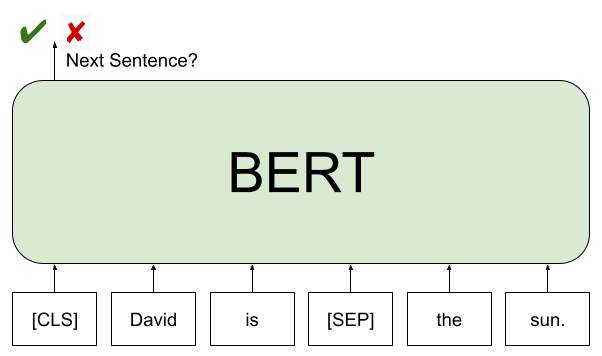
\includegraphics[width=0.9\textwidth]{images/illustrations/bert_nsp.png}
\caption{The illustration shows how the Next Sentence Prediciton (NSP) is implemented. The tokenizer adds a classifier and a separator token to the tokenized sentence pair. BERT then has to decide if the two sentence pairs belong to each other using the classifier token.}
\label{fig:bert_nsp}
\end{figure}

\paragraph{Next Sentence Prediction (NSP)}
The Next Sentence Prediction (NSP) task is a binary classification task. In section~\ref{sec:embeddings}, we have elaborated on the tokenizer. There is a special separator token, the [SEP] token. It separates a sequence of words or two sentences into two parts. BERT gets presented with either two matching parts or two parts that are not related to each other. During the training, BERT has to decide if the "next sentence" matches the previous one. It does so using the [CLS] token that the tokenizer adds to the beginning of every sequence. We present the basic architecture of this task in Figure~\ref{fig:bert_nsp}: An unlabeled sentence pair A and B serve as the input for the next sentence prediction. The tokenizer splits the words into tokens and adds a classifier and a separator token. After embedding the tokens into vectors and running them through the 12 transformer layers, BERT decides if the two-sentence pairs belong to each other. It does so using the classifier token at the first position of the output layer. 

\begin{figure}[htbp]
\centering
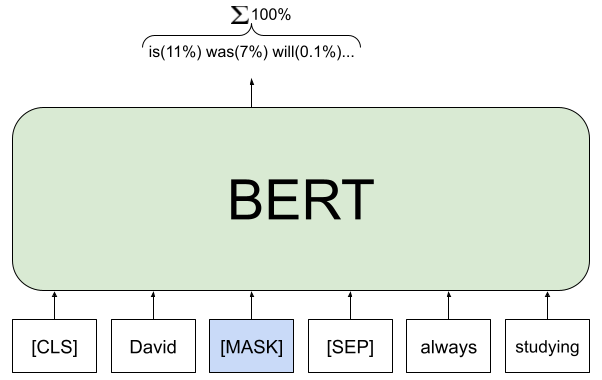
\includegraphics[width=0.9\textwidth]{images/illustrations/bert_mlm.png}
\caption{Depicted in the illustration is a simplified version of the Masked Language Model (MLM). Around 15\% of the word tokens get replaced with a mask token, and BERT has to predict the missing token. At the final output layer, BERT outputs a probability distribution that indicates how likely a word of the vocabulary is at the position of a masked token.}
\label{fig:bert_mlm}
\end{figure}

\paragraph{Masked Language Model (MLM)}
The Masked Language Model (MLM) task is essentially a guess the missing words task. During training, we replace random tokens with [MASK] tokens, and BERT has to predict these missing tokens. The vectors at the positions of the masked tokens at the final output layer get fed into a softmax function corresponding to the vocabulary. It produces a probability distribution that indicates how likely a word of the vocabulary is at the position of a masked token. In experimental results, the team at Google tried to determine the optimal percentage of tokens to mask and found that masking 15\% of the tokens is optimal. Figure~\ref{fig:bert_mlm} shows a simplified implementation of the task.


\section{BERT for Sequential Recommendations}\label{sec:bert_recommendations}
BERT was developed originally as a natural language model, and we have explained the architecture mainly in the context of word sequences. However, BERT has since found many more applications such as image classification, video classification, risk analysis, and investment advice~\cite{sun2019learning,heidari2020semantic,he2019hsi}.

The area we want to focus on is sequential recommendations. Learning and inferring information from sequences of text and sequences of user-item interactions are closely related tasks. Hence BERT is a good candidate for sequential recommendations and has shown state-of-the-art prediction results~\cite{sun2019bert4rec}. Recent applications of BERT include news recommendations, medical recommendations as well as course recommendations for students~\cite{shao2021degree,shang2019pre,jia2021rmbert}.

The use of BERT for recommendations was first described in the paper BERT4Rec, which we use as inspiration for our work~\cite{sun2019bert4rec}. We will now explain our custom implementation of BERT for sequential recommendations, including a custom tokenizer and custom pre-training using the Masked Language Model. 

\paragraph{Custom Tokenizer}
The first step in our custom tokenizer implementation is to build a vocabulary. We start by aggregating all unique items from all of the sequences of user-item interactions from our datasets. Items the user interacts with can be products, product reviews, or social media posts. We then give every item a unique number. The tokenizer turns each number in the vocabulary into a unique vector embedding, the input to the BERT model.

\paragraph{Custom Pre-Training}
Unlike many natural language models that only need a single custom output layer on top of a pre-trained BERT model, our implementation requires us to pre-train our model. Most BERT models are pre-trained using a vocabulary such as the English or Chinese language, whereas our model uses a custom vocabulary and tokenizer. For our custom pre-training, we will only use one of the BERT tasks: The Masked Language Model. In the original BERT paper, the authors compare the effect of pre-training with and without the Next Sentence Prediction task. The difference turned out to be very small, for some natural language processing challenges less than 0.1\% accuracy difference. Newer papers, that have experimented with modified BERT pre-training tasks have omitted the Next Sentence Prediction task entirely~\cite{yang2019xlnet,liu2019roberta}. We believe that the extra training time is not worth the potential small accuracy gain and that the Next Sentence Prediction task fits better in the context of language. Therefore we omit the task. 

\begin{figure}[htbp]
\centering
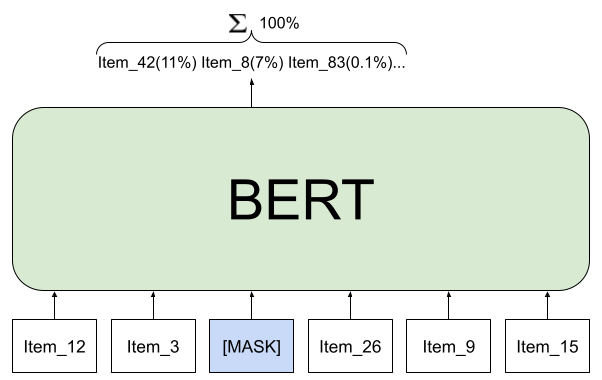
\includegraphics[width=0.9\textwidth]{images/illustrations/bert_custom.png}
\caption{The image shows our custom pre-training using the Masked Language Model. We mask random items in the sequence and BERT has to learn to predict them.}
\label{fig:bert_custom}
\end{figure}

We implement the Masked Language Model task to pre-train our model by masking random items in the sequences of user-item interactions. We follow the advice from the original BERT paper and mask 15\% of items. By predicting the missing items during pre-training, BERT learns which items users like and in what order they interact with the items. After pre-training, our BERT model can make accurate recommendations. For evaluation, we just mark the last item in every sequence and let BERT predict it, as explained in section~\ref{sec:test_procedure}. Depicted in Figure~\ref{fig:bert_custom} is an example of our custom pre-training.

% D.
% this whole chapter feels all super long and no wonder because we teach the reader lots of stuff all the time. All the teaching into the background. What's left is what we do. That's our system, what we sell.
% 